\chapter{Theoretical Foundations}
\label{theory}

I will start off by discussing the underlying architecture and theoretical models behind word2doc. Word2doc is made up of three
major components: First, InferSent, which is a sentence embedding method developed by Facebook \citep{infersent}, second a frequency
based document retriever also developed by Facebook and presented in \citep{drqa}, and finally the word2doc neural net architecture
itself, that I developed and present in this thesis. InferSent and the document retriever are a pre-processing step for the neural
network. Their results are combined and fed into the neural net, where the best fitting document is calculated. This
process is depicted in the figure below.

\begin{figure}[H]
  \begin{center}
    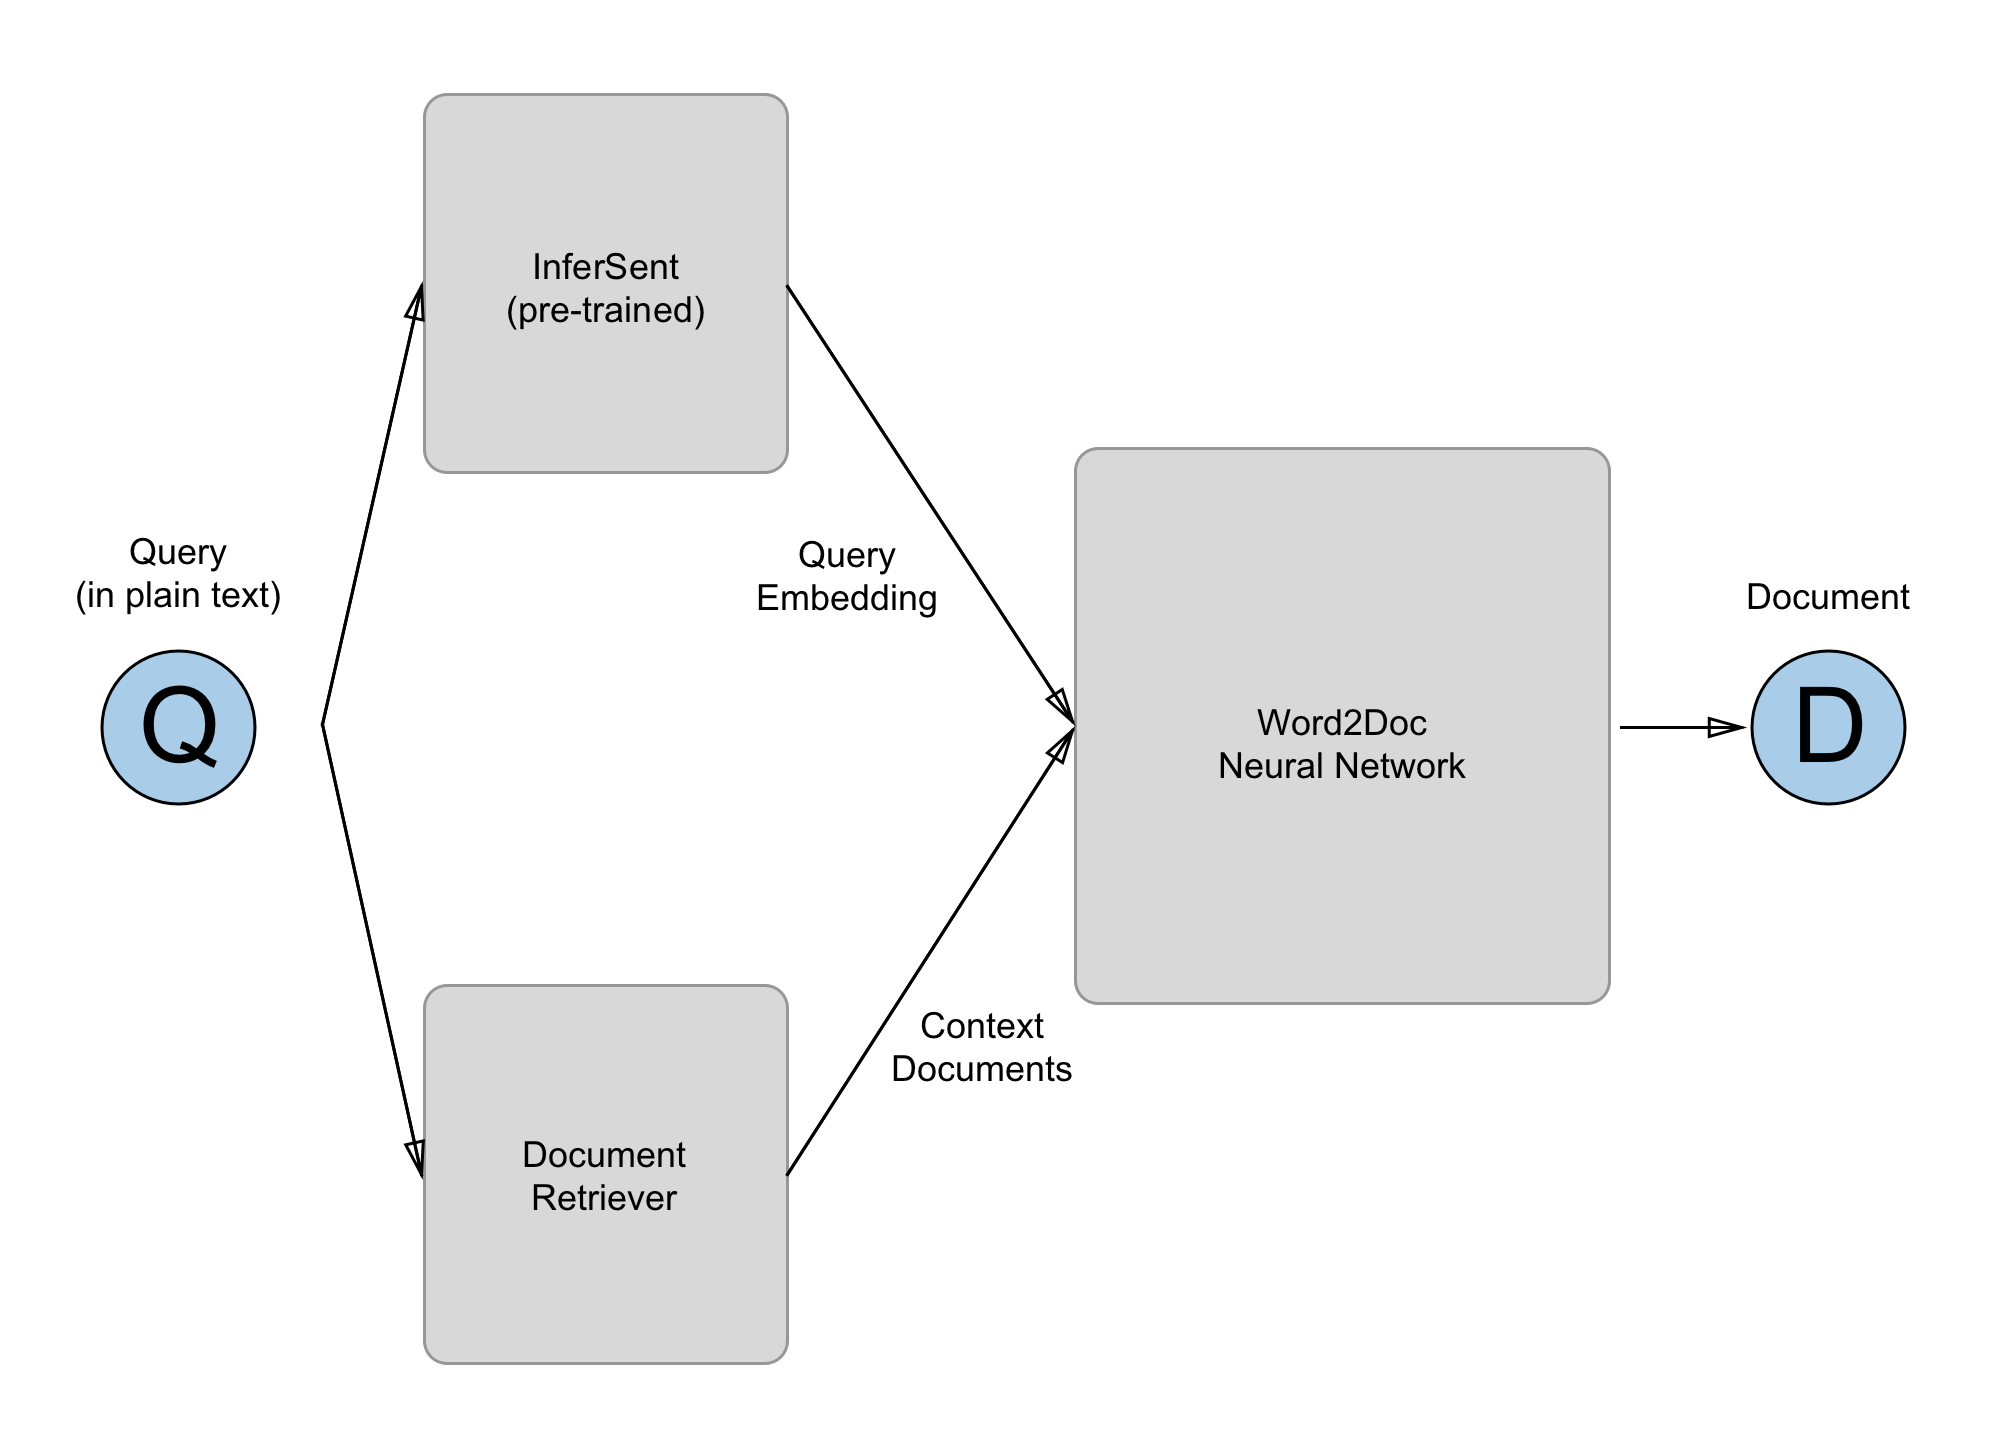
\includegraphics[scale=0.17]{W2D-Basic.png}
  \end{center}
  \caption{word2doc Overview}
  \medskip
  \label{fig:w2db}
\end{figure}

InferSent provides pre-trained sentence embeddings for the query. That means it generates an embedding out of the query, which is
called a \textit{query embedding}. Here, the query refers to the keyword or phrase we want to find a document for. I discuss this
process in depth in section \ref{theory:infersent}.

The document retriever generates a set of documents that are contextually similar to the one we are searching for. For example, say the
query consists of "football". Then the document retriever will find the ten most similar documents to football, which could be "soccer",
"goalie", etc. These documents provide the neural net with a context similar to the word contexts used to train word embeddings.
These documents are called \textit{context documents}.

Finally, the word2doc neural net takes both the query embedding and context documents as input to generate a final result, which is
the document best describing the initial query. In the following sections I will discuss each component in more detail. However,
first I will explain how word2doc is trained.


\subsubsection{Training}
\label{theory:training}

At prediction time, word2doc can take any query and return the best describing Wikipedia document, thus word2doc
operates on the entire English Wikipedia corpus. To achieve this, word2doc is also \textit{trained} on the entire Wikipedia corpus,
similar to the way word embeddings are trained on a specific corpus, and only function within that corpus. That means overfitting is
just as much a non-issue in word2doc as it is in word embeddings, since we want the model to represent as closely as possible the
distribution we are modeling.

More specifically, training data consists of the Wikipedia document title as the query and the document ID as the label, which I
also call the target document. Given the title, word2doc should learn to predict the document. However, as explained in section
\ref{sec:data}, the title is processed in such a way that word2doc doesn't memorize document-title pairs.


\section{Relevant Concepts}

Before I delve into more detail, I will explore some general concepts that will aid in the understanding of word2doc's full architecture.
Different kinds of embeddings play an important role in word2doc, and that is why I will briefly review the concept of an embedding,
and then explain sentence and document embeddings, which are more relevant for the thesis.


\subsection{Embeddings}
\label{theory:embb}

In the context of NLP, embeddings provide a means to compare the semantic similarity of two pieces of text. These pieces of text are
often single words, in which case the embedding is called a \textit{word embedding}. Their potential was arguably first demonstrated
by Collobert and Weston in \citet{coll-word-embb} and made popular through word2vec in \citet{word2vec}.

More specifically, an embedding is an \textit{n} dimensional vector representation of a piece of text, where the vector represents
the text's semantic meaning inside an \textit{n} dimensional vector space. For example, take three words, say king, queen and
apple, then the vectors for king and queen should lie closer to each other than the vectors for king and apple or queen and apple.
"Closer" refers to the distance between two vectors and it is measured by the cosine similarity, which I talk more about later.

The following well-known example offers an intuitive way to look at word embeddings. If you take a word embedding
for "king" and subtract the embedding for "man" and then add the embedding for "woman", the resulting vector will lie
closest to the vector representation for "queen" in the vector space. This is illustrated in Figure \ref{fig:w2vse}.

\begin{figure}
  \begin{center}
    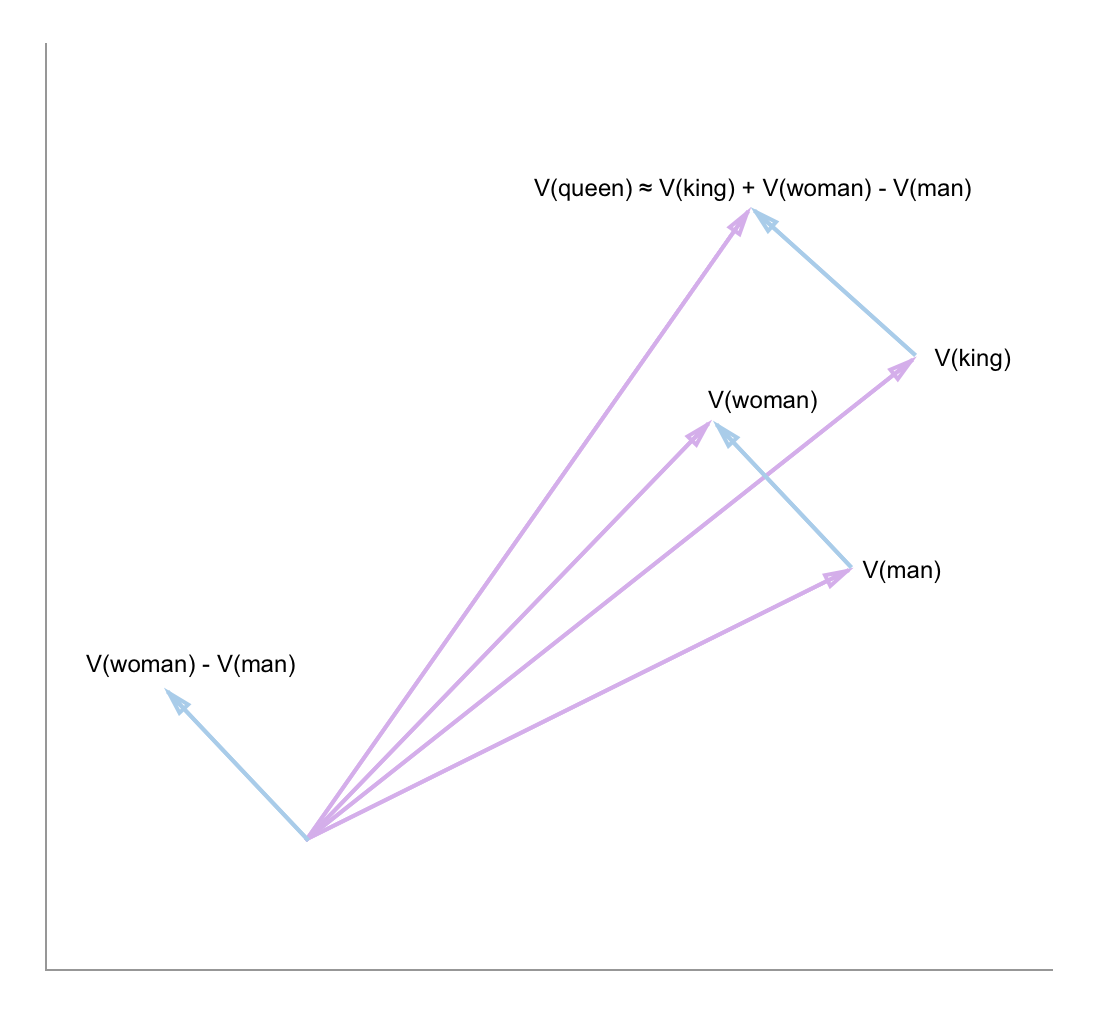
\includegraphics[scale=0.30]{word2vec-simp-ex.png}
  \end{center}
  \captionsetup{width=.75\linewidth}
  \caption{This figure shows possible calculations that can be done with word embeddings, and depicts in a simplified manner how
  embeddings represent semantic meaning. The \textit{V} functions calculates the embedding for a given word.}
  \label{fig:w2vse}
\end{figure}

Word embeddings are generally trained by scanning the context a word appears in. The context is defined as \textit{n} words that
surround the original word (a sort of window). If the network sees enough different word-context pairs, it will be able to
generalize and eventually learn the meaning of the word. How this works in detail is not relevant for this thesis, and suffice it
to say that there are two popular methods, one using the Bag-of-Words \citep{word2vec} approach and one using the skip-gram
approach \citep{neg-sample}.

It should also be noted that embeddings are low dimensional, meaning somewhere in the magnitude of 100s to 1000s. It turns out
there is a sweet spot for the dimensionality of an embedding: neither too small nor too large. This sort of phenomenon, which
can be found in many different machine learning problems, is often explained the following way: With too few parameters, the model
cannot fit the signal, but with too many parameters, the model starts overfitting. Surprisingly, I could not find a good theoretical
explanation to back up this intuition in the case of embeddings, so I will leave it at that. I mention this, because the low
dimensionality of word embeddings does play a role in their success, even if it is hard to explain why, and thus I chose the
magnitude for my embeddings accordingly.


\subsubsection{Sentence Embeddings}

Having reviewed embeddings, I will explain sentence embeddings. This is relevant in word2doc because the
query from Figure \ref{fig:w2db} is represented through such an embedding. This provides the neural network with a fixed
size semantic representation of the input query, which is easy for the network to work with.

The concept of a sentence embedding is very similar to the one of a word embedding. Instead of semantically
representing a single word, the embedding represents the semantic meaning of multiple words, thus of a phrase or a sentence. This does
become a significantly more complicated task and yields worse results than word embeddings, since much more goes into capturing the
semantics of a sentence compared to the semantics of a word. Word order, punctuation, and inflection all play a role in determining
the meaning of a sentence, which means sentences cannot be viewed as atomic elements, the way words can be.
However, there are some approaches to go about creating sentence embeddings that I will now discuss.

Many different techniques exist to calculate sentence embeddings, with methods ranging from simple arithmetical composition of the
word embeddings to more complex architectures using convolutional neural networks and recurrent neural networks.
(e.g., \citet{semb-eg1, skipthought, socher2011, blunsom2014, tai2015, wang2016})


\paragraph{Simple Arithmetical Compositions for Sentence Embeddings}

The first approach I will discuss is a simple additional composition of word vectors. As presented in \citet{semb-baseline},
computing the weighted average of individual word embeddings in the sentence and then removing the projections of the average vectors
on their first principal component, also known as common component removal, yields surprisingly promising results.

\citet{semb-baseline} further write that "...this method achieves significantly better performance than the unweighted
average on a variety of textual similarity tasks, and on most of these tasks even beats some sophisticated supervised methods tested
in \citet{wieting2016}, including some RNN and LSTM models." While this may be true, techniques based on compositions of
individual word embeddings have a drawback: they cannot handle out of vocabulary (OOV) words. If there is no pre-trained word
embedding for a given word in a sentence, then it is no longer possible to calculate the correct weighted average of all word
embeddings occurring in the sentence.

This is a cause of concern in the case of word2doc. It is likely that a word exists in the query for which there is no
pre-trained word embedding, especially since the query is most likely composed of complex and infrequently used words rather than
simple every day words. It is not an option to calculate pre-trained word embeddings for all possible queries because we cannot
know all possible future queries, and thus it is more than likely that a query contains one or more OOV words at some point.
As a result, the technique above is not a good option for word2doc, although it remains interesting for its simplicity.


\paragraph{Neural Net Approaches to Sentence Embeddings}

Another approach is presented in \citet{skipthought} as Skip-Thought Vectors, a method that uses an encoder-decoder architecture.
The encoder is an RNN that is trained to encode sentences as embeddings, and the decoder is consists of two RNNs that decode the
embeddings again into the two normal sentences that lie next to the original sentence. The idea is that sentences that lie next to
each other share context, and that correctly decoding sentences requires the embedding to contain enough contextual information of
the original sentence to be useful as an embedding. At the end, the decoders are thrown away and only the encoder is used to
generate sentence embeddings. This method has become very popular, yet it still suffers from out of vocabulary words.
To mitigate this problem, the authors present some methods of vocabulary expansion. For example, they propose working at
character level instead of word level.

All in all Skip-Thought Vectors could work for word2doc, however, the technique is outperformed by Facebook's InferSent
\citep{infersent} on various different tasks that measure the embedding's semantic representation.\footnote{For more information,
look at Table 4 in \citep{infersent}}. Furthermore, InferSent does not have any problems with OOV words.

\subsubsection{Document Embeddings}

Another form of embeddings are document embeddings. Just like other embeddings, document embeddings encode the semantic meaning
of an entire document inside a fixed length vector. In word2doc, a document embedding is calculated for every document in the
training data.

The document embeddings in word2doc are based on the paragraph vectors presented in \citet{doc2vec}. Yet, there are some relevant
changes that I made, however before I elaborate on those I will explain what paragraph vectors are.

\citet{doc2vec} present a way to calculate embeddings for paragraphs. They use a simple net that takes context words and a
paragraph (indexed by IDs) in the form of vectors as input, and that predicts the next word in the context. For example, the model
could take paragraph no. 42, "the", "cat", "sat", "on" as input and would try to predict "the". The architecture of that model is
illustrated in Figure \ref{fig:parvec}.

\begin{figure}
  \begin{center}
    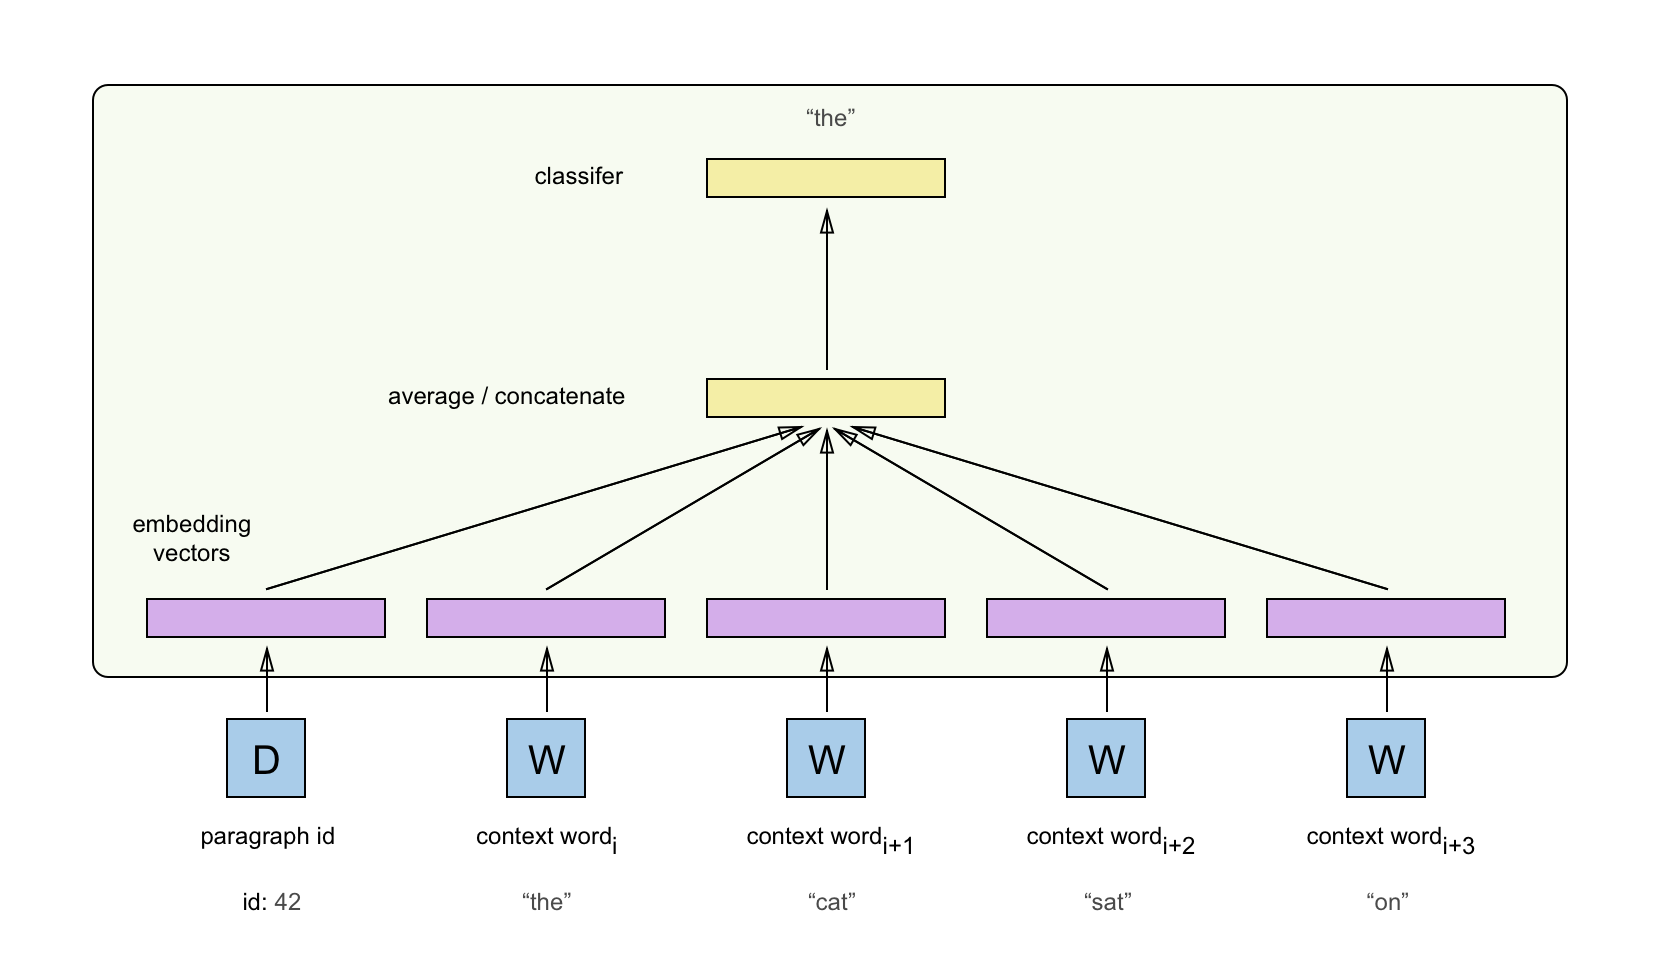
\includegraphics[scale=0.25]{doc2vec.png}
  \end{center}
  \captionsetup{width=.75\linewidth}
  \caption{The PV-DM framework for learning paragraph vectors from \citet{doc2vec}}
  \medskip
  \label{fig:parvec}
\end{figure}

At training, a paragraph is chosen, and a sliding window is used to slide over the paragraph. Every paragraph and word is mapped to
a unique vector, and as they are encountered again and again, these vectors are re-used. They slowly update their weights over the
duration of the training to reflect the semantic meaning of the word, similar to a word embedding. The downside is that each word
vector is kept the same across all seen paragraphs, which forces the net to generalize and thus learn.

At prediction time, the parameters for the model, the word vectors and the softmax weights, are fixed. Only the paragraph vector is
not fixed, and via gradient descent the values of the paragraph vector are calculated. This way, the model can predict a paragraph
vector for a never seen paragraph.

Word2doc does work differently than this as we will see later on, but it is inspired by this architecture.

\subsubsection{Distance Metric for Embeddings}
\label{theory:cosinesim}

In this section I will talk about how I measure the distance between two embeddings. In word2doc, I use the cosine similarity
metric, defined below.

\begin{gather}
similarity = cos(\theta) = \frac{A \cdot B}{\parallel A \parallel \parallel B \parallel}
\end{gather}

$A$ and $B$ are two vectors (the embeddings) and their dot product is divided by the product of their magnitudes. The result ranges
from -1 to 1, where -1 indicates exact opposites, 0 indicates orthogonality (not correlated) and 1 indicates they are exactly the same.

It is an open discussion whether cosine similarity is the best metric to use for this task. Cosine similarity uses the
norm of the vectors, and in doing so implicitly assumes the lengths of the vectors can be ignored, since they are normalized.
The norm of the vectors is a nice thing to use, because it is somewhat related to the overall frequency of which words occur in
the training corpus (in the case of word embeddings).\footnote{I could not find any solid evidence for this claim, however it seems to
be the general consensus among the community that it is so. This claim resurfaced on many GitHub issues and Stackoverflow posts
again and again.}

However, in practice it is not clear whether the length of the vectors can be ignored, or whether it might actually hide important
information and should be used. For example, \citet{schakelw15} argue that length does matter, and suggest using the L2 norm
in combination with term frequency to compare embeddings.

Despite this uncertainty, I chose the cosine similarity. Perhaps better results are possible with other methods, however cosine
similarity is by far the most established, and thus I deem it less risky compared to other methods.


\section{Architecture}

Now that I covered some basic concepts used in word2doc, I will talk about each system in word2doc in detail. As shown in
Figure \ref{fig:w2db} there are three major components, and I will start backwards, with the neural network itself, then explain
how InferSent works in detail and last explain the document retriever.


\subsection{word2doc Neural Network}
\label{theory:w2d-net}

In this section I will describe how the architecture of word2doc's neural net works. In a first step, I use a pre-trained model of
Facebook's InferSent \citep{infersent} to create a query embedding. So unlike in word2vec, the network does not take a word
as input, but rather a 4096 unit pre-trained sentence-embedding of the query (the query embedding). This allows the network to work
with any word, because InferSent can work with any OOV word, as explained above.

The network then takes this 4096-unit-long query embedding and trains a new fully connected hidden layer. The hidden layer's
purpose is to reduce the dimensions of the previous embedding, from 4096 to 512. This is done to reduce
the amount of work backpropagation has to do, since the amount of weights is drastically reduced. For example, look at the second
fully connected ReLu layer in Figure \ref{fig:w2d}. If we have 5 million units (so documents) in the output layer, and we keep the
4096 units instead of 512, then we would have to train $4096 * 5,000,000$ weights, close to 20 billion. Using 512 units
instead, we only have to train close to 2 billion weights, so considerably less.

Additionally, the network takes a list of context documents as input. This list of context documents is nothing
but a list of document IDs, so a list of integers. For each ID a document embedding is calculated in the same manner a word
embedding would be calculated. This implies that across all keywords, the document embeddings \textit{D} as seen in Figure
\ref{fig:w2d} stay the same for different keywords. It does not matter if the document 3234 appears in the context of the keyword
"football" or "quarterback", in both cases the same embedding will be used. This is important because it forces the network to
generalize. As the same document embeddings appear and re-appear in combination with different queries, their weights will
ultimately shift in a direction that reflects the semantic meaning of their documents.

All document embeddings are then averaged along with the output of the hidden layer from above,
similar to how it is discussed in the paragraph vectors from \citet{doc2vec}. However, in the case of paragraph vectors, the
authors concatenate instead of average, claiming that concatenation yielded better results. I also tested concatenation which I talk
about in section \ref{exp:dl}, however, word2doc yielded better results when averaging. Furthermore, the query embedding replaces
the paragraph id from Figure \ref{fig:parvec}, and the documents fetched by the document retriever replace the context
words used in paragraph vectors. That means instead of using a sliding window like it is done in paragraph vectors to identify
context, word2doc uses the document retriever. Additionally, the paragraph id that is trained in \citet{doc2vec} is used to make a
prediction that is kept instead of throwing it away. The interesting side effect is that that working document embeddings are
calculated this way. I talk more about this in section \ref{exp:embb}.

The concatenation is then passed into another fully connected ReLu layer to reduce the dimensions again for the same reason as
above. This reduced tensor is then passed to the output layer, where a one-hot encoding is calculated using negative sampling (a
loss function) to find the best matching document. See Figure \ref{fig:w2d}.

\begin{sidewaysfigure}
  \begin{center}
    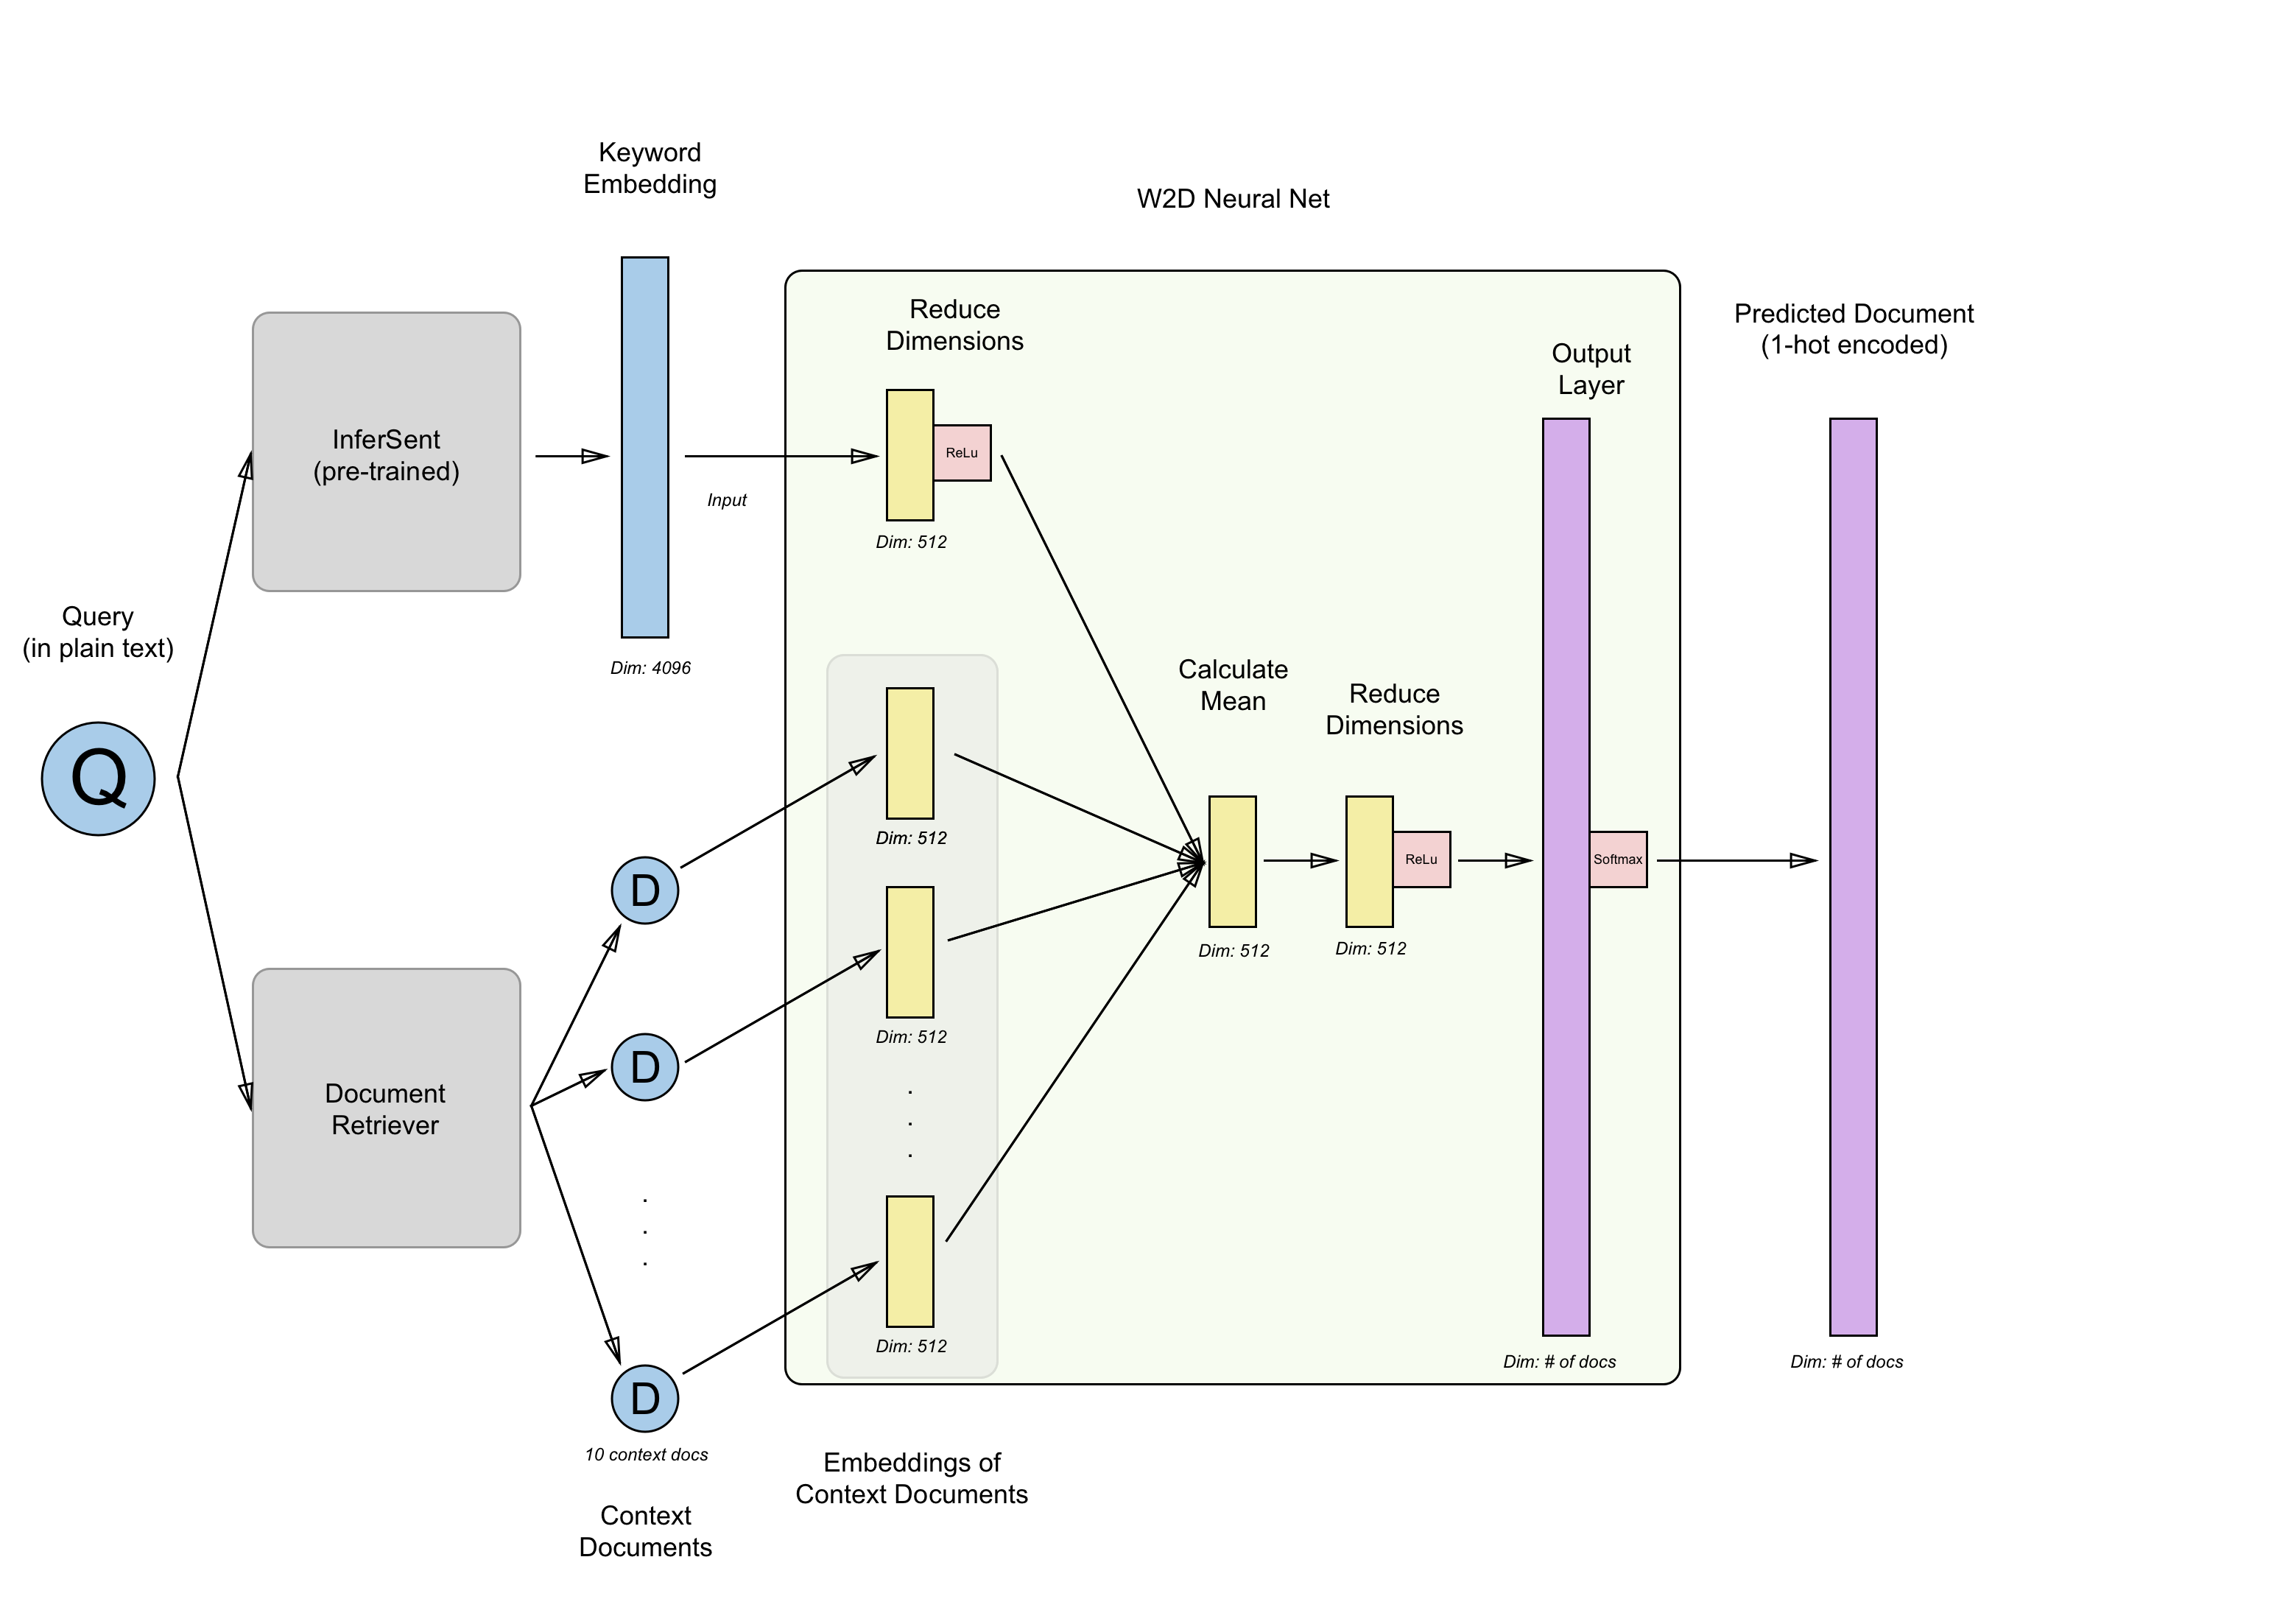
\includegraphics[scale=0.17]{W2DV.png}
  \end{center}
  \caption{W2D Architecture}
  \label{fig:w2d}
\end{sidewaysfigure}


\subsubsection{Negative Sampling}
\label{theory:negsamp}
Word2doc uses negative sampling as a loss function. Negative sampling is a technique proposed by \citet{neg-sample} to speed up
training. Instead of adjusting all weights of the final output layer in each iteration, only a handful of weights are updated.
A small amount of "negative" keywords are chosen, keywords that have nothing to do with the actual "positive" keyword.
For example, if "neural network" is the positive keyword, then "gardening" and "football" might be negative keywords, because
they have nothing to do with "neural network". The weights for the positive keyword are then updated in a "positive" direction,
and the weights for the negative keywords are updated in a "negative" direction.

If done over many iterations, negative sampling will eventually update all weights while being much faster than the
classic approach. Since word2doc has the total number of Wikipedia articles as output neurons, negative sampling is necessary,
otherwise training would take a very long time.

Usually negative samples are chosen through the frequency of their occurrence, with more frequent words being more likely to be
chosen as negative samples. In the case of word2doc however, there is no meaningful probability that a given query occurs.
As a result, the network is handed a subset of documents (the context documents) from which not to sample, and it samples
randomly from all other remaining documents.

\subsection{InferSent}
\label{theory:inf}

As mentioned before, Infersent is a tool used to calculate sentence embeddings developed by Facebook \citep{infersent}.
In word2doc it is used to create sentence embeddings from the query in order to get a fixed
size semantic representation of all possible queries. The resulting embedding has a dimension of 4096, and is fed into the neural
network where it is combined with context documents to choose a final, best matching document to the query. In this section I
explain how this is done in detail.

\citet{infersent} investigate seven different sentence encoding architectures, and find out that
"...an encoder based on a bi-directional LSTM architecture with max pooling, trained on the Stanford Natural Language Inference (SNLI)
dataset \citep{bowmanAPM15}, yields state-of-the-art sentence embeddings compared to all existing alternative unsupervised
approaches like SkipThought or FastSent, while being much faster to train." Furthermore, they note, "...we establish this finding on a
broad and diverse set of transfer tasks that measures the ability of sentence representations to capture general and useful
information."

A transfer task is a problem in which knowledge gained in one task is applied to another. For example, knowledge
gained while learning to recognize cars could be applied when trying to recognize trucks. This is what word2doc needs to be able to
do. During training, queries are created through augmented Wikipedia titles and keywords, yet at prediction word2doc needs to
handle more abstract and complicated queries created by people. Thus, Wikipedia titles are learned and need to be applied to a more
general, real-life scenario. Granted, this is not as clear as the car and truck example from above, but it still qualifies
nonetheless. Thus, if InferSent does well on transfer tasks, it should do well for word2doc.


Furthermore, InferSent uses the SNLI dataset as training data, which, the authors theorize, works well with sentence embeddings.

\begin{quote}
The SNLI dataset consists of 512k human-generated English sentence pairs, manually labeled with one
of three categories: entailment, contradiction and neutral. It captures natural language inference, also known in previous
incarnations as Recognizing Textual Entailment (RTE), and constitutes one of the largest high-quality labeled resources explicitly
constructed in order to require understanding sentence semantics. We hypothesize that the semantic nature of NLI makes it a good
candidate for learning universal sentence embeddings in a supervised way. That is, we aim to demonstrate that sentence encoders
trained on natural language inference are able to learn sentence representations that capture universally useful features.
\end{quote} \citep{infersent}

The sample data from the SNLI corpus is shown in Table \ref{tbl:snli}, taken from the SNLI website.
\footnote{Note that this is not the exact representation. Some details were left out for the sake of simplicity. For the exact
representation, please visit \href{https://nlp.stanford.edu/projects/snli/}{https://nlp.stanford.edu/projects/snli}}

\begin{table}
  \centering
  \begin{tabular}{|p{5cm}|p{3cm}|p{5cm}|}
    \hline
    \multicolumn{3}{|c|}{SNLI Sample Data} \\
    \hline
    Premise&Judgment&Hypothesis \\
    \hline
    \hline
    A man inspects the uniform of a figure in some East Asian country & contradiction & The man is sleeping \\
    A smiling costumed woman is holding an umbrella & neutral & A happy woman in a fairy costume holds an umbrella \\
    A black race car starts up in front of a crowd of people & contradiction & A man is driving down a lonely road \\
    A soccer game with multiple males playing & entailment &	Some men are playing a sport \\
    \hline
  \end{tabular}
  \caption{SNLI Sample Data}
  \label{tbl:snli}
\end{table}

\subsubsection{InferSent Architecture}
\label{theory:infersent}

The basic architecture is illustrated in Figure \ref{fig:inf1} on the next page. The architecture has two sentence encoders that output a
representation for the premise $u$ and the hypothesis $v$. Once the resulting sentence vectors are generated, relations between
$u$ and $v$ are calculated using three methods: concatenation, element-wise product and absolute element-wise difference. The
result is fed into a 3-class classifier consisting of multiple fully connected layers culminating in a softmax layer. The network
is trained to predict the judgment between the premise and the hypothesis.

\begin{figure}
  \begin{center}
    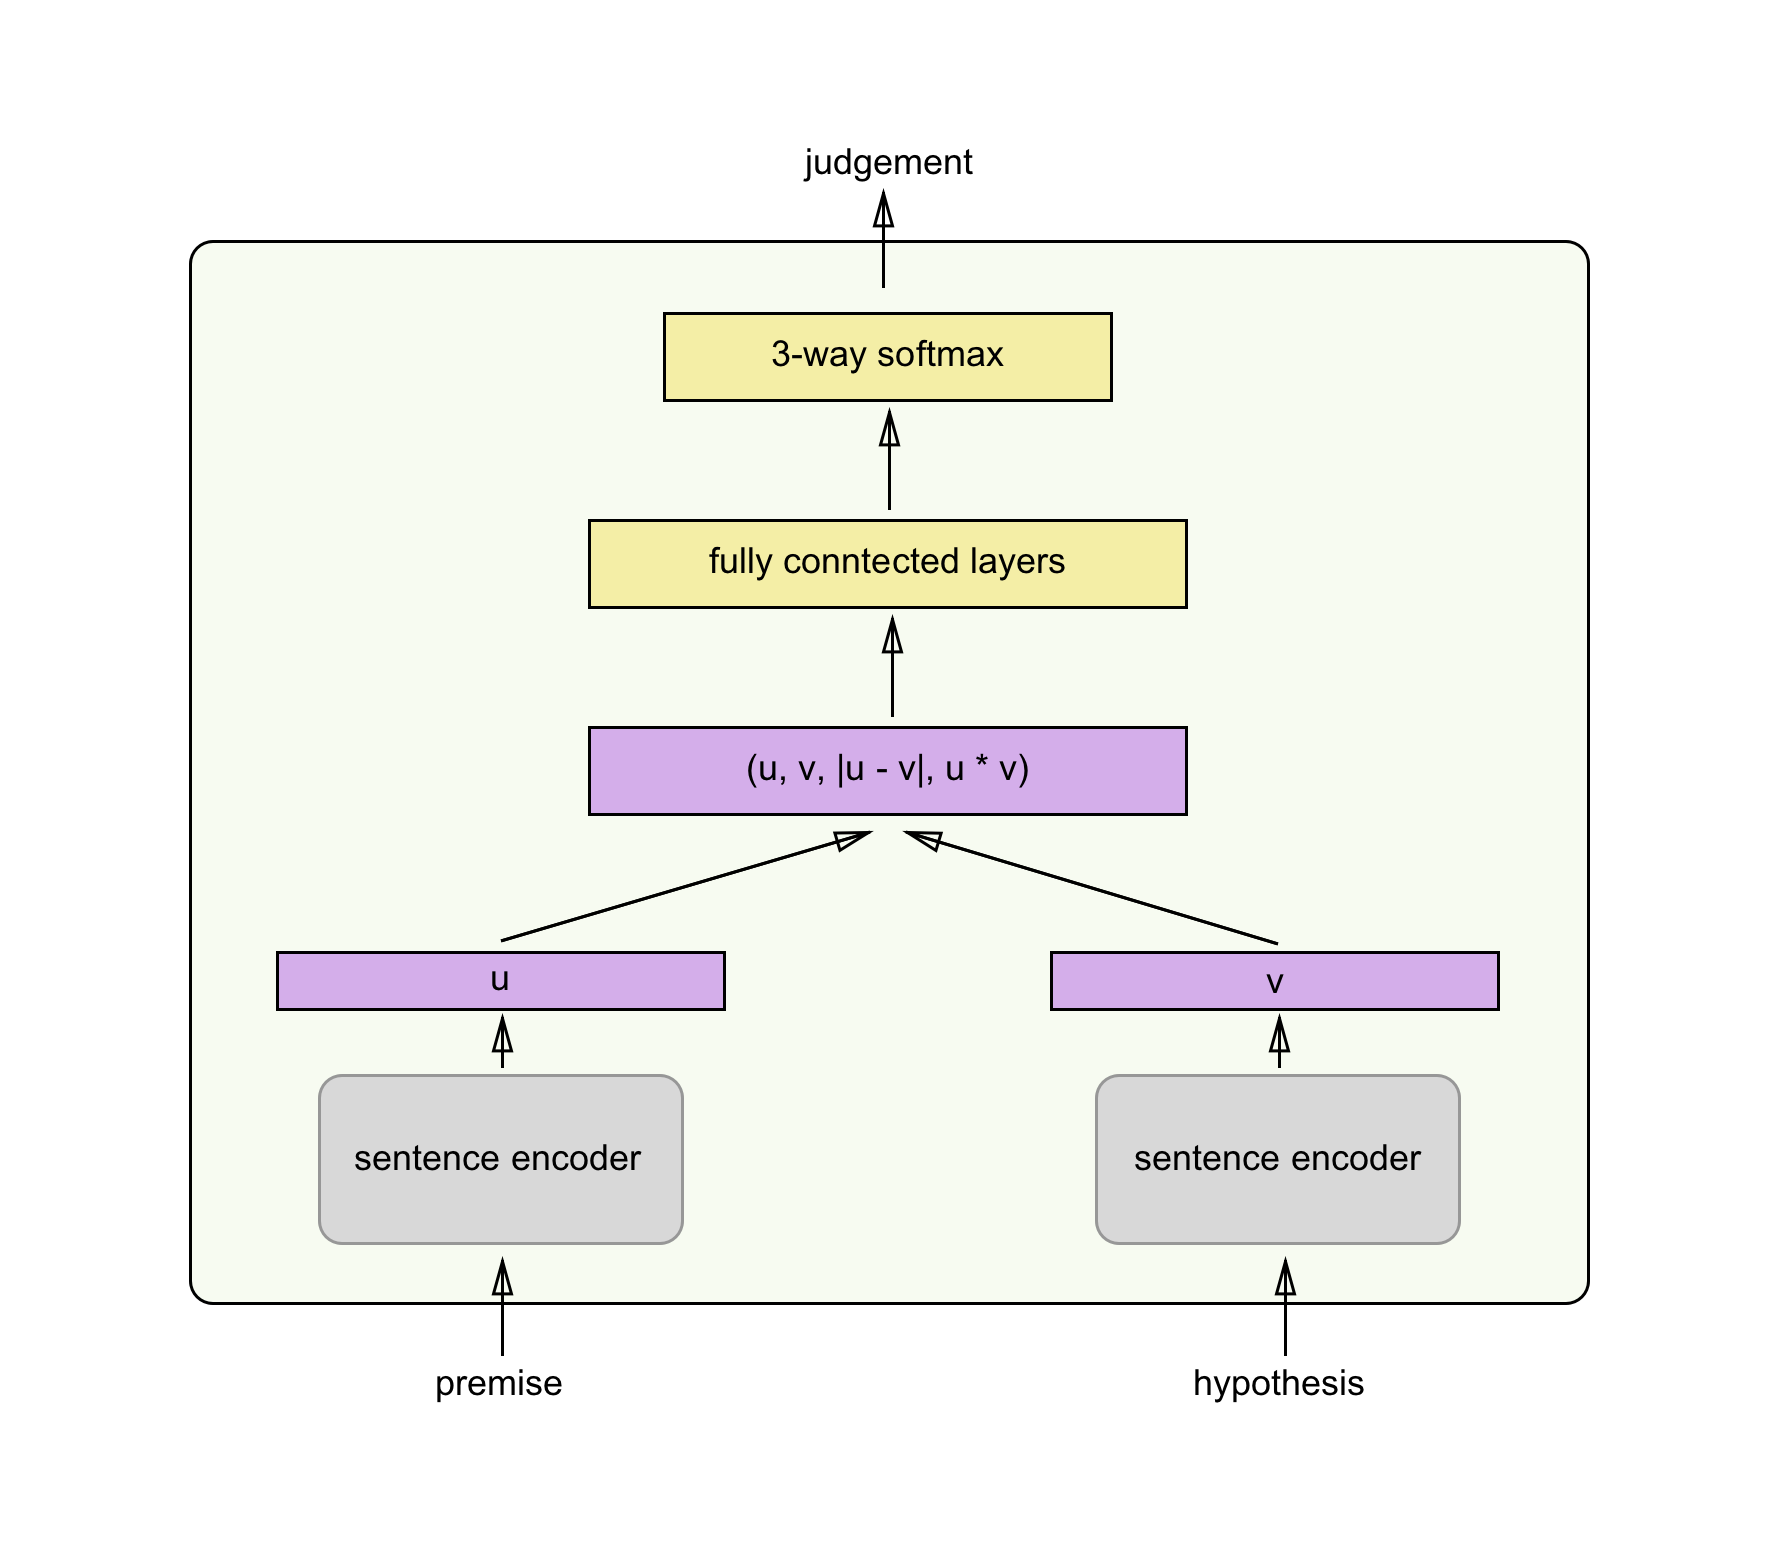
\includegraphics[scale=0.15]{infersent-generic-nli.png}
  \end{center}
  \captionsetup{width=.75\linewidth}
  \caption{InferSent Natural Language Inference Training Scheme based on Figure 1 in \citet{infersent}}
  \label{fig:inf1}
\end{figure}

Next, I will talk about the sentence encoder. Like I mentioned in the beginning of this section, the authors of InferSent tested
seven different sentence encoder models, and found out that the bi-directional LSTM architecture with max pooling performed
the best. Thus, I will ignore the other methods and only focus on the bi-directional LSTM here.

Two LSTMs read a sequence of words from the premise and hypothesis in opposing directions, generating the vectors $h_t$ by
concatenating the forward and backward LSTMs in the following way \citep{infersent}:

\begin{gather}
\overrightarrow{h_t} = \overrightarrow{LSTM}_t(w_1,...,w_T) \\
\overleftarrow{h_t} = \overleftarrow{LSTM}_t(w_1,...,w_T) \\
h_t = [\overrightarrow{h_t}, \overleftarrow{h_t}]
\end{gather}

That means $h_t$ is the concatenation of $\overrightarrow{h_t}$ and $\overleftarrow{h_t}$. The $h_t$s are then combined through
max-pooling \citep{max-pooling}, a technique in which the maximum value over each dimension of the hidden units in the LSTM is
selected. This is illustrated in the Figure \ref{fig:inf3} from the original paper.

\begin{figure}
  \begin{center}
    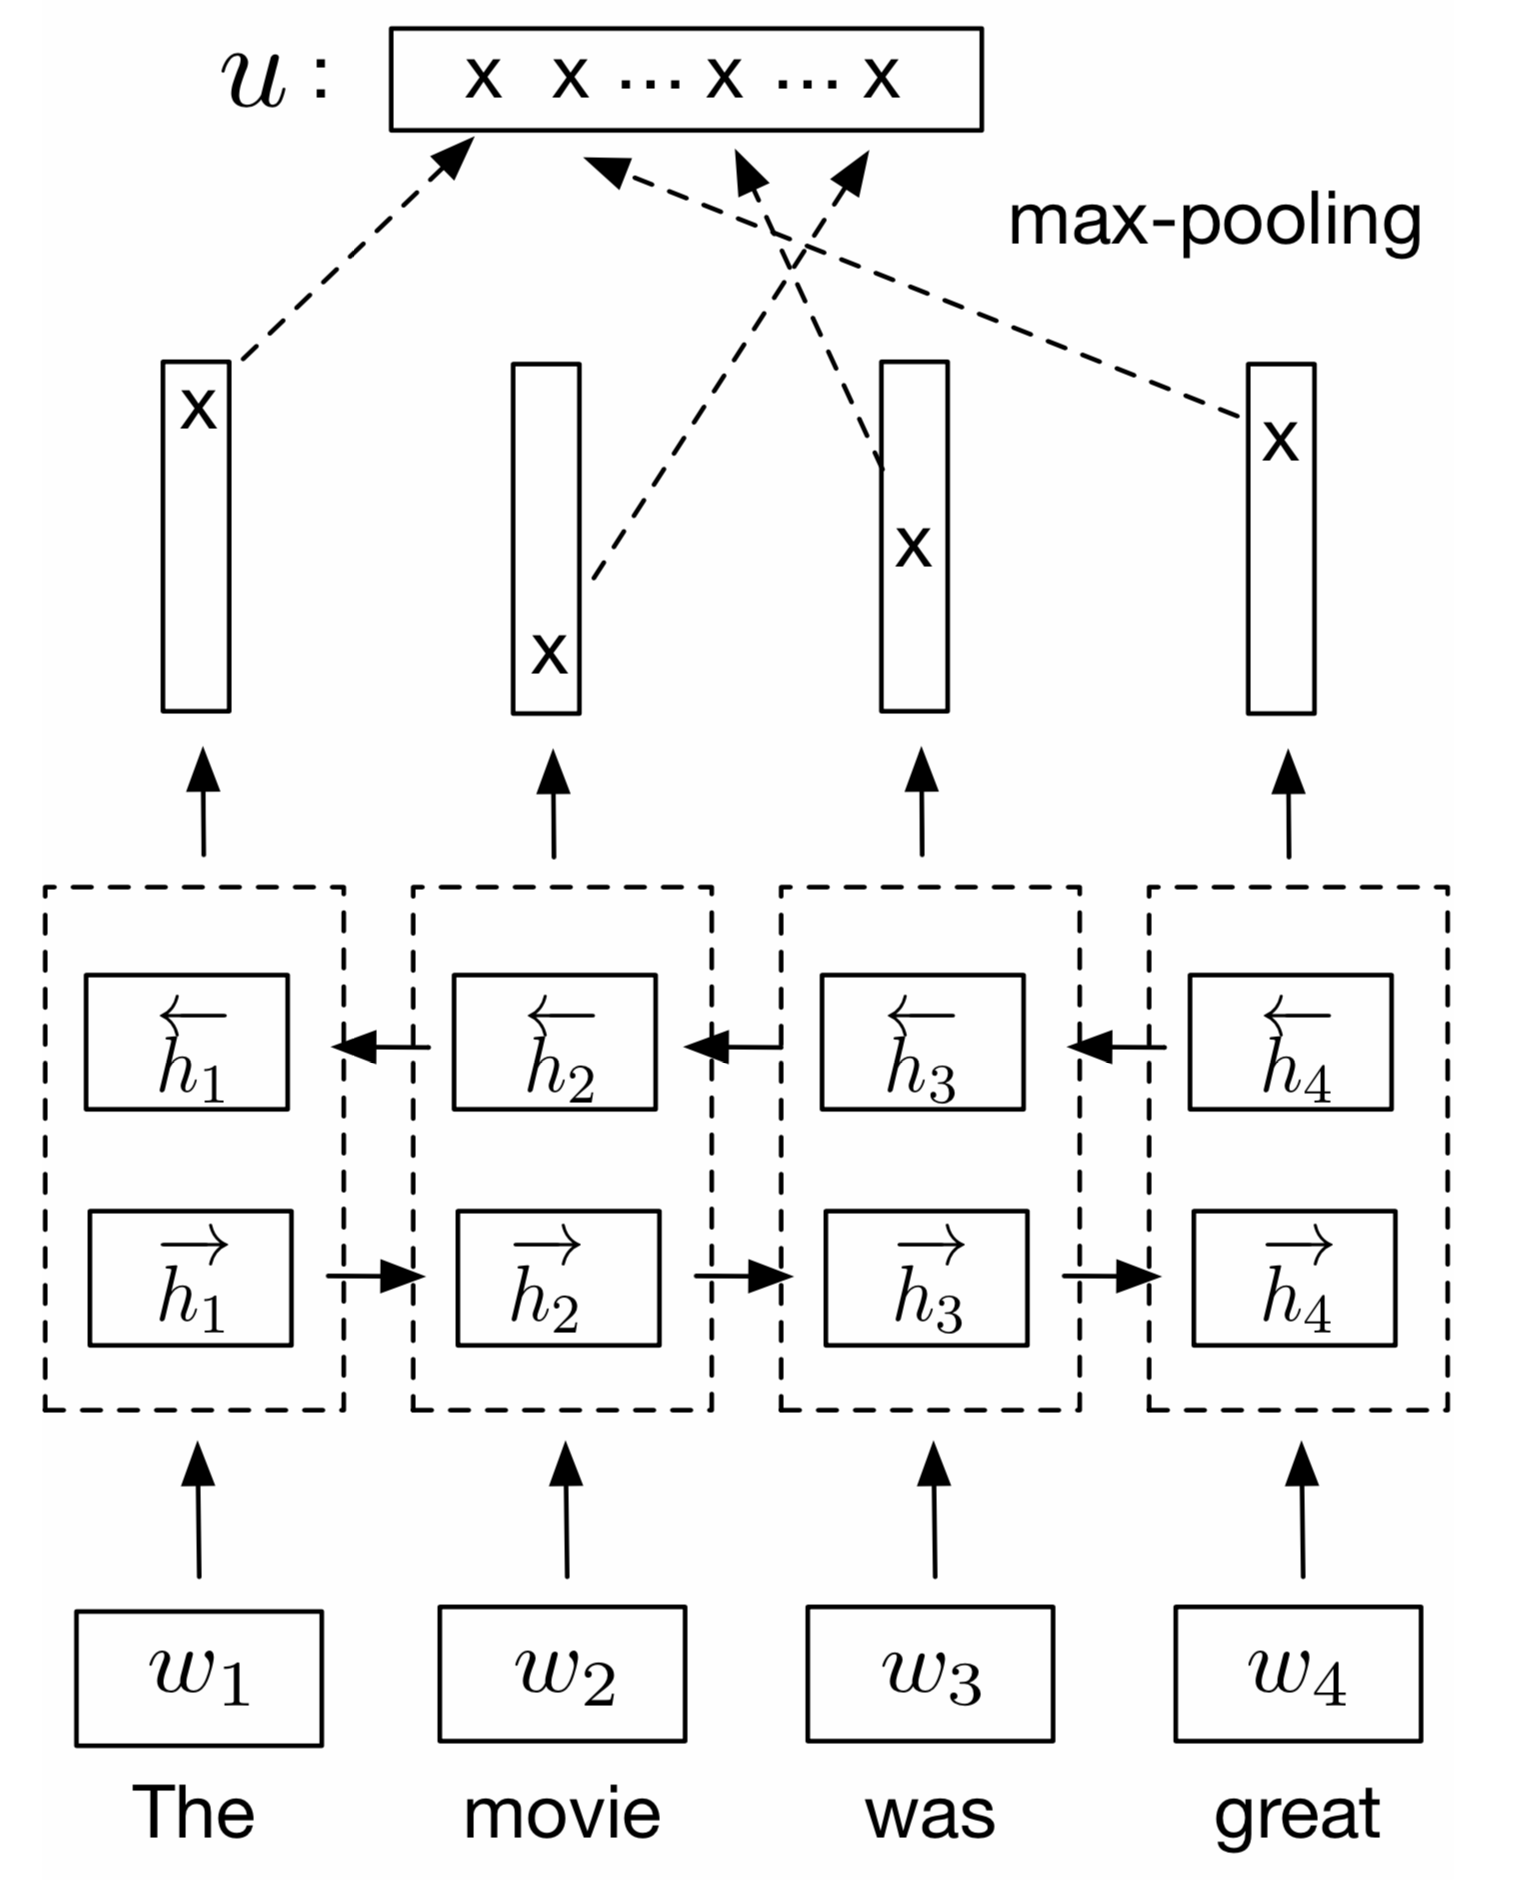
\includegraphics[scale=0.18]{bi-lstm.png}
  \end{center}
  \captionsetup{width=.75\linewidth}
  \caption{Bi-directional LSTM used as sentence encoder (Figure 2 in \citet{infersent})}
  \label{fig:inf3}
\end{figure}

The result of this max pooling operation then yields the finished sentence encoding that is plugged back into the model seen in
Figure \ref{fig:inf1}.


\subsection{Document Retriever}
\label{theory:docret}

The document retriever is taken from Facebook's DrQA system \citep{drqa} and it replaces the sliding
window from paragraph vectors \citep{doc2vec} to generate a list of contextually similar documents that match the query. In
this section I will explain how this is done.

The document retriever takes the query as input, and generates a list of ten documents that best match the query. Best in this
context means documents that are closest to the query's topic. You can find an example of what this looks like in Table
\ref{tbl:doc-ret} on the next page.

\begin{table}
  \centering
  \begin{tabular}{|p{3cm}|p{7cm}|}
    \hline
    \multicolumn{2}{|c|}{Document Retriever Sample Results} \\
    \hline
    Query&"neural nets"\\
    \hline
    Results&Convolutional neural network\\
    (as Wikipedia&Deep learning\\
    document names)&Alternative explanations of the "grandmother" cell\\
    &The Age of Spiritual Machines\\
    &Artificial neural network\\
    &History of artificial intelligence \\
    &Artificial consciousness\\
    &Deeplearning4j\\
    &Speech recognition\\
    &Neurophilosophy\\
    \hline
  \end{tabular}
  \caption{Document Retriever Sample Results}
  \label{tbl:doc-ret}
\end{table}

Table \ref{tbl:doc-ret} shows the actual results when submitting "neural nets" to the document retriever.
They are listed in no particular order, because order does not matter in word2doc, as they are shuffled
before training.

These documents are calculated purely through a non-machine-learning technique that is based on the frequencies of occurring words
from the query. In a first step, an inverted index is created using all Wikipedia documents. More specifically, a sparse word to
document count matrix $M$ is created, such that $M_{ij}$ is the number of times word $i$ appears in document $j$. Word $i$ is in
fact not quite a word, but the hash of a bigram. This is done, according to the authors, to take local word order into account,
which further improves the system by 1-2\%. The authors note, that bigrams provided the best results out of all tried n-grams.
\footnote{Unfortunetaly, the authors of \citet{drqa} do not provide data as to what other n-grams they tested.}
An unsigned \textit{murmur3} hash function \citep{weinberger2009} is used to quickly count the number of times a
bigram appears in a document by dividing it into $2^{24}$ bins, which preserves speed and memory.

After this word count matrix is calculated, it is transformed into a TF-IDF matrix. TF-IDF is a numerical statistic that reflects
to a certain degree how important a word is to a document within a corpus of documents. The TF-IDF value for a word changes
proportionally to the frequency of the word in a document and is offset by the frequency of the word in the corpus, which takes
into account that some words appear more frequently in general. The bigger this value, the more "important" the word is in the
document, and the smaller the value, the less "important" it is. Thus, every element in the count matrix is transformed the following
way to get a TF-IDF filled document matrix $M'$.

\begin{gather}
tfidf = log(tf + 1) * log((N - N_t + 0.5) / (N_t + 0.5))
\end{gather}

$tf$ is the term frequency, $N$ is the number of documents and $N_t$ is the number of times term $t$ occurs in all documents. Thus,
a term frequency based model is calculated, but note that term still refers to bigrams, and not unigrams.

Finally, a TF-IDF-weighted word vector $V$ is calculated from the query, and the dot product between it and the TF-IDF document
matrix is calculated in the vector space the of the TF-IDF-weighted word vector. To calculate $V$, the query is essentially seen as
its own document, and the entire process from above is repeated for this new "document". Thus, we get a vector of TF-IDF weighted
bigrams from the query.

The dot product between $V$ and the TF-IDF document matrix $M'$ is then formed the following way: Since there are $2^{24}$ bins,
and since there are 5,316,954 documents in the Wikipedia dump I am using, $M'$ has dimensions of $2^{24} x 5,316,954$. The word
vector $V$, like $M$, is also sparse and since its bigrams are subject to the same hash function system, its bigrams are also put
into bins of size $2^{24}$. Thus, it has the dimensions of $|V| x 2^{24}$, where $|V|$ is the number of bigrams created from the
query, so the length of $V$. Since $V$ and $M'$ share a dimension, the dot product can be calculated between the two, and the
result is a sparse matrix $R$ of size $1 x 5,316,954$, essentially a vector of document scores for each document. Finally, the top
ten biggest scores from $R$ are taken, and the documents belonging to the scores are returned as the best matching documents.
Theses are the results in Table \ref{tbl:doc-ret}.

Taking the dot product between $V$ and $M'$ works because high TF-IDF scores from the query ("important" bigrams to the query)
multiplied with high TF-IDF scores from a document ("important" bigrams to the document) yield a high product overall. If this
happens with enough bigrams throughout the document, and is not offset by low TF-IDF score products, the sum of all of these
scores (the dot product) will be rather high too, signaling that this document is a potential match for this query. If however, the
query and the document do not contextually match well, there should be a considerable amount of bigrams whose product does not
yield high scores, and thus the overall score is diminished compared to cases in which the query and document contextually do match.

